\documentclass[serif,mathserif]{beamer}
\usepackage{color}
\definecolor{mycolor}{rgb}{0.5, 0.5, 0.5}
\usepackage{amsmath, amsfonts, epsfig, xspace}
\usepackage{algorithm,algorithmic}
\usepackage{pstricks,pst-node}
\usepackage{multimedia}
\usepackage[normal,tight,center]{subfigure}
\setlength{\subfigcapskip}{-.5em}
\usepackage{beamerthemesplit}
\usetheme{keynote}
\usepackage{/Library/Frameworks/R.framework/Resources/share/texmf/Sweave}

%Flow Diagrams
\usepackage{tikz}
\usetikzlibrary{positioning,shapes.geometric}


\title[Community Genetics
  Model \hspace{2em}\insertframenumber]{Interaction Network Structure
  in Community Genetics}

\subtitle{A Genes to Ecosystem Model}
\author[]{\textbf{Matthew K. Lau$^1$},\\ S.R. Borrett$^2$, T.G. Whitham$^1$}
\date{}
\institute[\url{http://dana.ucc.nau.edu/~mkl48/bio/home.html}]{
Northern Arizona University$^1$ \\
University of North Carolina$^2$
}
\begin{document}
\setkeys{Gin}{width=0.6\textwidth}

\frame{\titlepage}

% \section{Introduction}  % add these to see outline in slides



\begin{frame}
  \frametitle{Main Questions:}
  \begin{enumerate}
  \item What is the structure of genotype-genotype networks? 
    \begin{enumerate}
    \item trait variation (matching)
    \item mobility
    \item space
    \item demography (death rate)
    \item ???
    \end{enumerate}
  \item How does genotype-genotype network structure influence the
    evolution of species and network architecture?
    \begin{enumerate}
    \item random
    \item nested
    \item modular
    \item centralized
    \item ???
    \end{enumerate}
  \item How does genotype-genotype network structure influence
    ecological structure?
    \begin{enumerate}
    \item species abundance curves
    \item genotype-species networks
    \end{enumerate}
  \end{enumerate}
\end{frame}


\begin{frame}
  \frametitle{Key Points}
  \begin{itemize}
  \item Understanding the effect of the structure of ecological
    networks on evolutionary dynamics is important in communities of
    interacting species (Van Ommeren and Whitham, Ulanowicz) \pause
  \item Here, I present the framework for a genes to ecosystem model
    that will allow us to investigate how interaction network 
    structure affects: \pause
    \begin{enumerate}
      \item the evolutionary response of the community to selection on
        a focal species \pause
      \item the stability of the community in terms of the resistance
        and resilience of the community \pause
      \item the covariance of traits in different species \pause
    \end{enumerate}
%  \item From another perspective, the model's intent is to explore how network structure affects
%    the spread of evolutionary shifts within a community? \pause
  \item The primary focus is to introduce or remove variables within
    the current model framework \pause
  \end{itemize}
\end{frame}

%What is the question?

\begin{frame}
  \frametitle{What is the significance of networks to community genetics?}
  \begin{itemize}
  \item Using genetics to predict the structure and dynamics of communities  \pause
  \item Indirect effects and feedbacks in communities complicate the
    influence of foundation species \pause
  \item Network theory provides scalable predictions for complex
    systems: \pause
    \begin{itemize}
    \item Food webs with more connections will tend to be more stable
      (MacArthur 1955) \pause
    \item Complexity increases instability in random networks (May
      1972) \pause
    \item Network architecture influences dynamics:
      \begin{enumerate}
      \item World Wide Web (Albert, Jeong and Barab\'{a}si 2000) \pause
      \item Mutualistic networks (Bascompte et al. 2003) \pause
      \item Food webs (Dunne, Williams and Martinez 2004) \pause
      \end{enumerate}
    \end{itemize}
  \end{itemize}
\end{frame}

\begin{frame}
  \frametitle{Evolution ``OF'' Networks}

  \begin{columns}
    \begin{column}{.5\linewidth}
      \begin{center}
        \begin{tikzpicture}[%
            -,shorten >=0pt,>=stealth,node distance=1cm,
            noname/.style={%
              ellipse,minimum width=1.25em,minimum height=1.25em,draw
            }
          ]
          \node[noname,fill=green] (1)                          {};
          \node[noname,fill=green] (2) [below of=1]             {};
          \node[noname,fill=green] (3) [below of=2]             {};
          \node[noname,fill=red] (4)   [right of=1]             {};
          \node[noname,fill=red] (5)   [below of=4]             {};
          \node[noname,fill=red] (6)   [below of=5]             {};

          \path 
          (1) edge                   node {} (4) 
          (1) edge                   node {} (5) 
          (1) edge                   node {} (6) 
          (2) edge                   node {} (5) 
          (3) edge                   node {} (6) 
          ;
        \end{tikzpicture}
        \\
        $t$
      \end{center}
    \end{column}
    \begin{column}{.5\linewidth}
      \begin{center}
        \begin{tikzpicture}[%
            -,shorten >=0pt,>=stealth,node distance=1cm,
            noname/.style={%
              ellipse,minimum width=1.25em,minimum height=1.25em,draw
            }
          ]
          \node[noname,fill=green] (1)                          {};
          \node[noname,fill=green] (2) [below of=1]             {};
          \node[noname,fill=green] (3) [below of=2]             {};
          \node[noname,fill=red] (4)   [right of=1]             {};
          \node[noname,fill=red] (5)   [below of=4]             {};
          \node[noname,fill=red] (6)   [below of=5]             {};

          \path 
          (1) edge                   node {} (4) 
          (2) edge                   node {} (5) 
          (3) edge                   node {} (4) 
          (3) edge                   node {} (5) 
          (3) edge                   node {} (6) 
          ;
        \end{tikzpicture}
        \\
        $t + 1$
      \end{center}
    \end{column}
  \end{columns}
  \begin{center}
    Interaction traits evolve and change network architecture.
  \end{center}
\end{frame}

\begin{frame}
  \frametitle{Evolution ``ON'' Networks}
  \begin{columns}
    \begin{column}{.5\linewidth}
      \begin{center}
        \begin{tikzpicture}[%
            -,shorten >=0pt,>=stealth,node distance=1cm,
            noname/.style={%
              ellipse,minimum width=1.25em,minimum height=1.25em,draw
            }
          ]
          \node[noname,fill=green] (1)                          {};
          \node[noname,fill=green] (2) [below of=1]             {};
          \node[noname,fill=green] (3) [below of=2]             {};
          \node[noname,fill=red] (4)   [right of=1]             {};
          \node[noname,fill=red] (5)   [below of=4]             {};
          \node[noname,fill=red] (6)   [below of=5]             {};

          \path 
          (1) edge                   node {} (4) 
          (1) edge                   node {} (5) 
          (1) edge                   node {} (6) 
          (2) edge                   node {} (5) 
          (3) edge                   node {} (6) 
          ;
        \end{tikzpicture}
      \end{center}
    \end{column}
    \begin{column}{.5\linewidth}
      \begin{center}
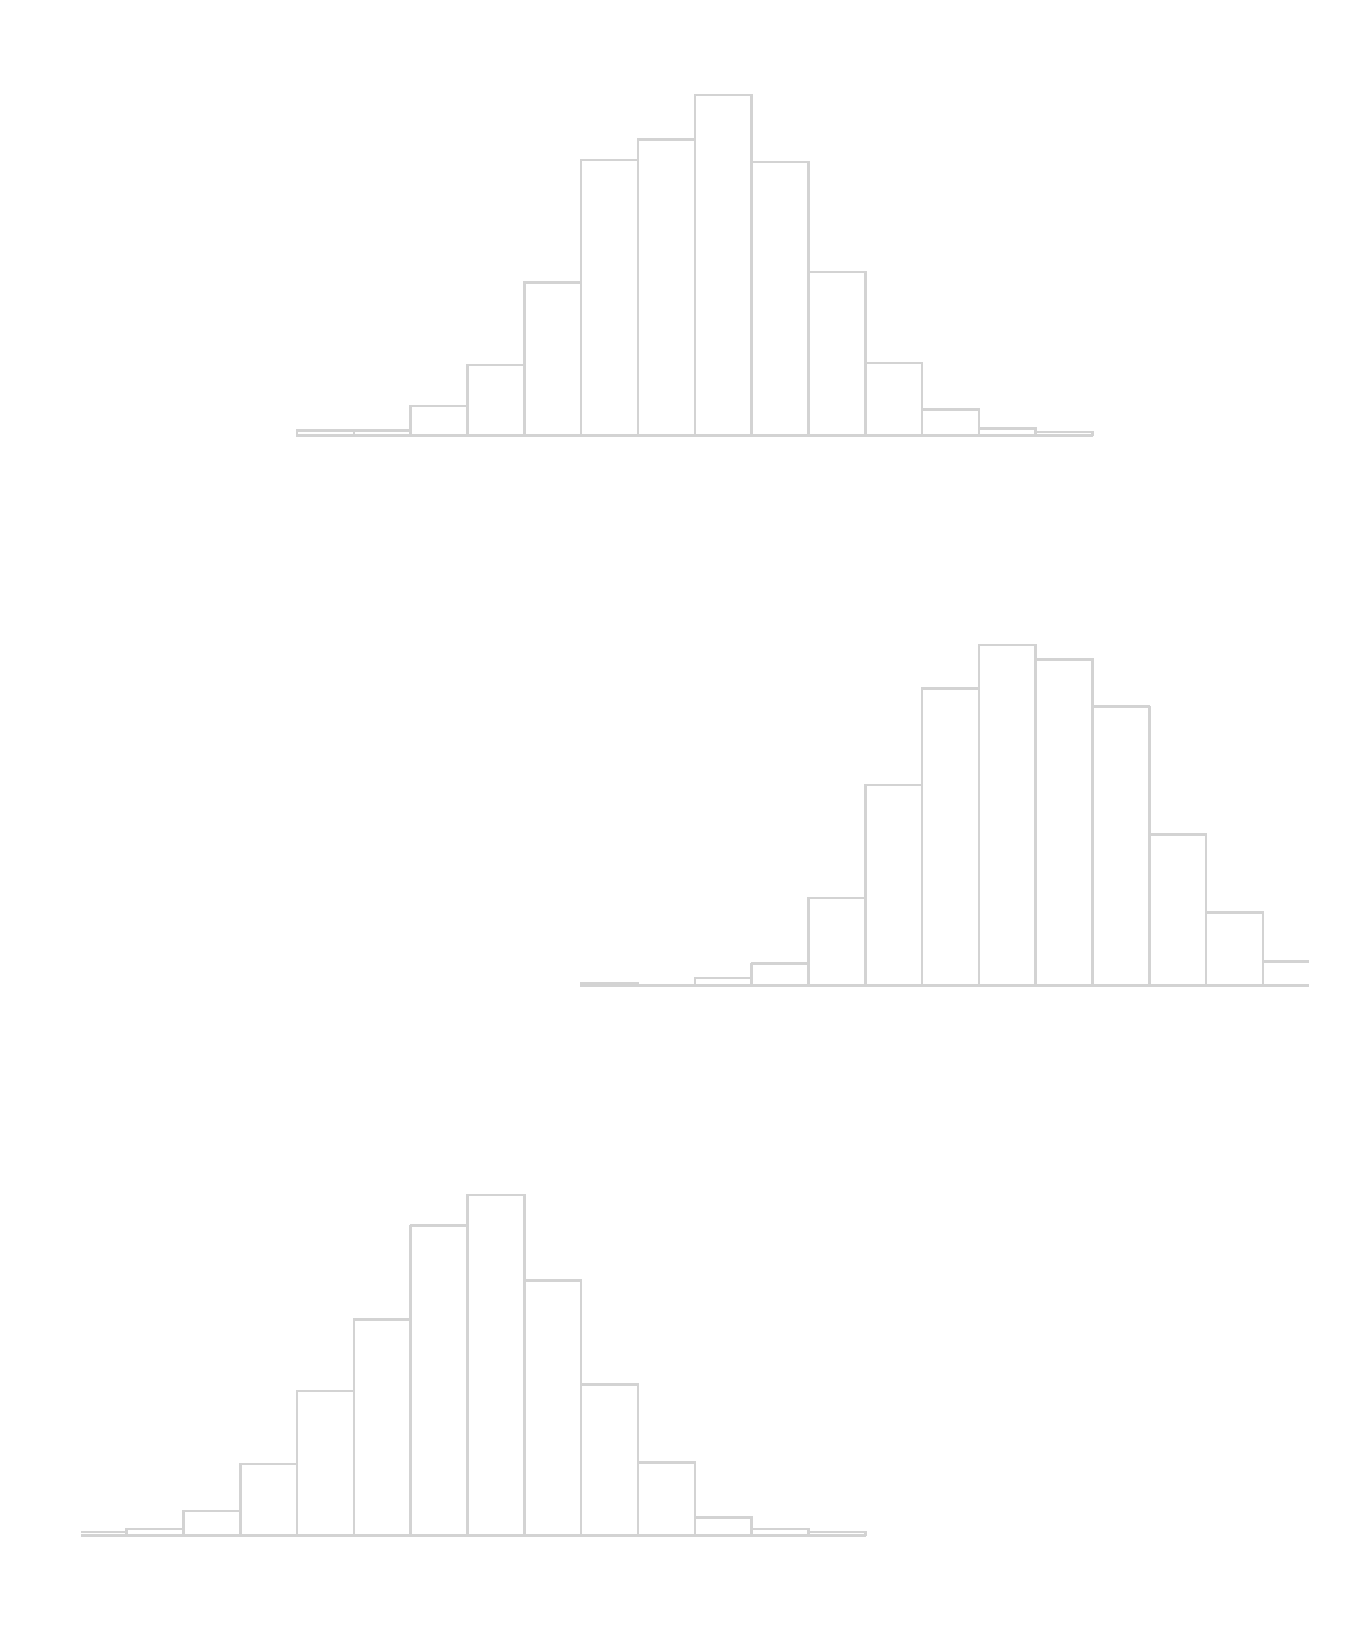
\includegraphics{presentation-001}
      \end{center}
    \end{column}
  \end{columns}
  \begin{center}
    Traits (interactions or otherwise) evolve from direct and indirect selection.
  \end{center}
\end{frame}


%Why should we care?


\begin{frame}
  \frametitle{Selection on Networks}
  \begin{center}
    \begin{tikzpicture}[%
        ->,
        shorten >=2pt,
        >=stealth,
        node distance=1cm,
        noname/.style={%
          ellipse,
          minimum width=5em,
          minimum height=3em,
          draw
        }
      ]
      \node[noname] (1)              {Genotype 1};
      \node[noname] (3) [right=of 1] {Herbivore};
      \node[noname] (4) [right=of 3] {Predator};
      \node[noname] (2) [node distance=2cm, below=of 1] {Genotype 2};
      \node[noname] (5) [right=of 2] {Herbivore};
      \node[noname] (6) [right=of 5] {Predator};
      \path 
      (1) edge  [above, bend left=20pt]                 node {+} (3) 
      (1) edge  [above,bend left=35pt] node {--} (4) 
      (3) edge  [above, bend left=20pt]                 node {--} (1)
      (3) edge  [above, bend left=20pt]                 node {+} (4)
      (4) edge  [above, bend left=20pt]                 node {--} (3)
%
      (2) edge  [above, bend left=20pt]                 node {+} (5)
      (5) edge  [above, bend left=20pt]                 node {--} (2)
      (5) edge  [above, bend left=20pt]                 node {+} (6)
      (6) edge  [above, bend left=20pt]                 node {--} (5)
      (2) edge  [above,bend left=35pt]                  node {+} (6) 
;
    \end{tikzpicture}
  \end{center}
\end{frame}


\begin{frame}
  \frametitle{Selection on Networks}
  \begin{center}
    \begin{tikzpicture}[%
        ->,
        shorten >=2pt,
        >=stealth,
        node distance=1cm,
        noname/.style={%
          ellipse,
          minimum width=5em,
          minimum height=3em,
          draw
        }
      ]
      \node[noname] (1)              {Genotype 1};
      \node[noname] (3) [right=of 1] {Herbivore};
      \node[noname] (4) [right=of 3] {Predator};
      \node[noname] (2) [node distance=2cm, below=of 1] {Genotype 2};
      \node[noname] (5) [right=of 2] {Herbivore};
      \node[noname] (6) [right=of 5] {Predator};
      \path 
      (1) edge  [above, bend left=20pt]                 node {+} (3) 
      (3) edge  [above, bend left=20pt]                 node {--} (1)
      (3) edge  [above, bend left=20pt]                 node {+} (4)
      (4) edge  [above, bend left=20pt]                 node {--} (3)
      (1) edge  [above,bend left=35pt]                  node {\huge \textbf{--}} (4) 
%
      (2) edge  [above, bend left=20pt]                 node {+} (5)
      (5) edge  [above, bend left=20pt]                 node {--} (2)
      (5) edge  [above, bend left=20pt]                 node {+} (6)
      (6) edge  [above, bend left=20pt]                 node {--} (5)
      (2) edge  [above,bend left=35pt]                  node {\huge \textbf{+}} (6) 
;
    \end{tikzpicture}
  \end{center}
\end{frame}

\begin{frame}
  \frametitle{Selection on Networks}
  \begin{center}
    \begin{tikzpicture}[%
        ->,
        shorten >=2pt,
        >=stealth,
        node distance=1cm,
        noname/.style={%
          ellipse,
          minimum width=5em,
          minimum height=3em,
          draw
        }
      ]
      \node[noname] (1)              {Genotype 1};
      \node[noname] (3) [right=of 1] {Herbivore};
      \node[noname] (4) [right=of 3] {Predator};
      \node[noname] (2) [node distance=2.5cm, below=of 1] {Genotype 2};
      \node[noname] (5) [right=of 2] {Herbivore};
      \node[noname] (6) [right=of 5] {Predator};
      \path 
      (1) edge  [above, bend left=20pt]                 node {+} (3) 
      (3) edge  [above, bend left=20pt]                 node {--} (1)
      (3) edge  [above, bend left=20pt]                 node {+} (4)
      (4) edge  [above, bend left=20pt]                 node {--} (3)
      (1) edge  [above,bend left=35pt]                  node {\huge \textbf{--}} (4) 
      (4) edge  [dashed,above,bend left=30pt]           node {} (1) 
%
      (2) edge  [above, bend left=20pt]                 node {+} (5)
      (5) edge  [above, bend left=20pt]                 node {--} (2)
      (5) edge  [above, bend left=20pt]                 node {+} (6)
      (6) edge  [above, bend left=20pt]                 node {--} (5)
      (2) edge  [above,bend left=35pt]                  node {\huge \textbf{+}} (6) 
      (6) edge  [dashed,above,bend left=30pt]           node {} (2) 
;
    \end{tikzpicture}
  \end{center}
\end{frame}

\begin{frame}
  \frametitle{Selection on Networks}
  \begin{center}
    \begin{tikzpicture}[%
        ->,
        shorten >=2pt,
        >=stealth,
        node distance=1cm,
        noname/.style={%
          ellipse,
          minimum width=5em,
          minimum height=3em,
          draw
        }
      ]
      \node[noname] (1)              {Genotype 1};
      \node[noname] (3) [right=of 1] {};
      \node[noname] (4) [right=of 3] {Predator};
      \node[noname] (2) [node distance=2.5cm, below=of 1] {Genotype 2};
      \node[noname] (5) [right=of 2] {};
      \node[noname] (6) [right=of 5] {Predator};
      \path 
      (1) edge  [above,bend left=30pt]                  node {\huge \textbf{--}} (4) 
      (4) edge  [dashed,above,bend left=40pt]           node {\huge \textbf{+}} (1) 
%
      (2) edge  [above,bend left=30pt]                  node {\huge \textbf{+}} (6) 
      (6) edge  [dashed,above,bend left=40pt]           node {\huge \textbf{+}} (2) 
;
    \end{tikzpicture}
  \end{center}
\end{frame}

%What's been done?
\begin{frame}
  \frametitle{Where are we at?}
  \begin{itemize}
  \item Papers from our group:  \pause
    \begin{itemize}
    \item Dixon's paper
    \item Wimp's paper
    \item Martinsen's paper
    \item Bailey's paper
    \item Bridgeland's paper
    \item Shuster et al. 2006
    \item Lonsdorf (unpublished)
    \end{itemize}
  \item Papers from other community genetics groups: \pause
    \begin{itemize}
    \item Agrawal
    \item Mooney (ant-aphid-plant)
    \item Genung (Genetic variation and community change – selection,
      evolution, and feedbacks)
    \end{itemize}
  \item Papers on network evolution:
    \begin{itemize}
    \item ?????
    \end{itemize}
  \end{itemize}
\end{frame}

%Why use modeling?
\begin{frame}
  \frametitle{Why model?}
  \begin{itemize}
  \item General principals  \pause
  \item Generate hypotheses  \pause
  \item Quantitative predictions 
  \end{itemize}
\end{frame}


%Flow diagram of model
%Model process

\begin{frame}
  \frametitle{Framework}
  \begin{center}
    \begin{tikzpicture}[%
        ->,shorten >=2pt,>=stealth,node distance=1cm,
        noname/.style={%
          ellipse,minimum width=5em,minimum height=3em,draw
        }
      ]
      \node[noname] (1)              {G};
      \node[noname] (2) [below=of 1] {P};
      \node[noname] (3) [right=of 2] {E};
      \node[noname] (4) [right=of 3] {F};
      \node[noname] (5) [above=of 4] {R};
      \path 
      (1) edge                   node {} (2) 
      (2) edge                   node {} (3)
      (3) edge                   node {} (4)
      (4) edge                      node {} (5)
      (5) edge  [bend right=20pt]   node {} (1);
    \end{tikzpicture}
  \end{center}
  \begin{center}
    \begin{columns}
      \begin{column}{.5\linewidth}
        \begin{itemize}
        \item G = genotype
        \item P = phenotype
        \item E = ecology
        \end{itemize}
      \end{column}
      \begin{column}{.5\linewidth}
        \begin{itemize}
        \item F = fitness
        \item R = reproduction
        \item 
        \end{itemize}
      \end{column}
    \end{columns}
  \end{center}    
\end{frame}

%Implementation
\begin{frame}
  \frametitle{Implementation}
  \begin{itemize}
  \item Differential Equations (Mass Action)
  \item Individual Based Models (IBM)
  \end{itemize}
\end{frame}

\begin{frame}
  \frametitle{Implementation: What is an IBM?}
  \begin{itemize}
  \item Specify the core system processes 
  \item Emergent properties 
  \item Computationally intensive (tracking individuals) 
  \end{itemize}
\end{frame}

\begin{frame}
  \frametitle{Implementation: Genotype}
  \begin{itemize}
    \item Binary sequence
    \item Ploidy
  \end{itemize}
\end{frame}

\begin{frame}
  \frametitle{Implementation: Phenotype}
  \begin{itemize}
    \item Initiate from random population means
    \item Dominance
    \item Epistasis
  \end{itemize}
\end{frame}

\begin{frame}
  \frametitle{Implementation: Ecology}
  \begin{itemize}
    \item Networks 
      \begin{itemize}
      \item Centrality
      \item Nestedness
      \item Modularity
      \end{itemize}
  \item Relative abundance
  \item Resource limitation
  \item Abiotic
  \item Space?
  \end{itemize}
\end{frame}

\begin{frame}
  \frametitle{Implementation: Fitness}
  \begin{itemize}
  \item Trait Matching (resource) 
  \item Resistance (trophic)
  \end{itemize}
\end{frame}

\begin{frame}
  \frametitle{Implementation: Reproduction}
  \begin{itemize}
  \item Demographics (death + birth - ?carrying capacity?)
  \item Recombination (based on relative fitness distribution)
  \item Mutation
  \item Hybridization
  \end{itemize}
\end{frame}

\begin{frame}
  \frametitle{Framework}
  \begin{center}
    \begin{tikzpicture}[%
        ->,shorten >=2pt,>=stealth,node distance=1cm,
        noname/.style={%
          ellipse,minimum width=5em,minimum height=3em,draw
        }
      ]
      \node[noname] (1)              {G};
      \node[noname] (2) [below=of 1] {P};
      \node[noname] (3) [right=of 2] {E};
      \node[noname] (4) [right=of 3] {F};
      \node[noname] (5) [above=of 4] {R};
      \path 
      (1) edge                   node {} (2) 
      (2) edge                   node {} (3)
      (3) edge                   node {} (4)
      (4) edge                      node {} (5)
      (5) edge  [bend right=20pt]   node {} (1);
    \end{tikzpicture}
  \end{center}
  \begin{center}
    \begin{columns}
      \begin{column}{.5\linewidth}
        \begin{itemize}
        \item G = genotype
        \item P = phenotype
        \item E = ecology
        \end{itemize}
      \end{column}
      \begin{column}{.5\linewidth}
        \begin{itemize}
        \item F = fitness
        \item R = reproduction
        \item 
        \end{itemize}
      \end{column}
    \end{columns}
  \end{center}    
\end{frame}

\begin{frame}
  \frametitle{Framework}
  \begin{center}
    \begin{tikzpicture}[%
        ->,shorten >=2pt,>=stealth,node distance=1cm,
        noname/.style={%
          ellipse,minimum width=5em,minimum height=3em,draw
        }
      ]
      \node[noname] (1)              {G};
      \node[noname] (2) [below=of 1] {P};
      \node[noname] (3) [right=of 2] {E};
      \node[noname] (4) [right=of 3] {F};
      \node[noname] (5) [above=of 4] {R};
      \node[noname] (6) [circle,node distance=1.5cm,above of = 3,minimum size=1.5] {\huge \textbf{S}};
      \path 
      (1) edge                   node {} (2) 
      (2) edge                   node {} (3)
      (3) edge                   node {} (4)
      (4) edge                      node {} (5)
      (5) edge  [bend right=20pt]   node {} (1);
    \end{tikzpicture}
  \end{center}
  \begin{center}
    \begin{columns}
      \begin{column}{.5\linewidth}
        \begin{itemize}
        \item G = genotype
        \item P = phenotype
        \item E = ecology
        \end{itemize}
      \end{column}
      \begin{column}{.5\linewidth}
        \begin{itemize}
        \item F = fitness
        \item R = reproduction
        \item \textbf{S = selection}
        \end{itemize}
      \end{column}
    \end{columns}
  \end{center}
\end{frame}

\begin{frame}
  \frametitle{Implementation: Selection}
  \begin{itemize}
  \item Add a species (preferential attachment)
  \item Remove individuals
  \item Shift resource availability
  \item Evolve resistance
  \end{itemize}
\end{frame}


\begin{frame}
  \frametitle{Implementation: Computation}
  \begin{itemize}
  \item Bioinformatics Server?  
  \item Other suggestions?  
  \end{itemize}
\end{frame}


%% \begin{frame}
%%   \frametitle{}
%%   \begin{itemize}
%%   \item   \pause
%%   \end{itemize}
%% \end{frame}

%% \begin{frame}
%%   \frametitle{}
%%   \begin{itemize}
%%   \item   \pause
%%   \end{itemize}
%% \end{frame}


%% %including pictures
%% \begin{frame}
%%   \frametitle{}
%%   \begin{figure}[h!]
%%     \centering
%%     \includegraphics[width=11cm]{figures/ONC_close.jpg}
%%   \end{figure}
%% \end{frame}


\begin{frame}
  \frametitle{Acknowledgments}
  \begin{itemize}
  \item A.K. Salas (UT Austin) \& the SEE Lab (UNCW)
  \item E. Lonsdorf (Chicago Botanic Garden) \& S. Shuster (NAU)
  \item M. Fortuna \& J. Bascompte (Estaci\'{o}n Biol\'{o}gica
    de Do\~{n}ana)
  \item Open Source Software: \textbf{R}, emacs and \LaTeX
  \end{itemize}
\end{frame}


\begin{frame}
  \frametitle{}
%%The End.
\end{frame}


%% \begin{frame}
%%   \frametitle{}
%%   \begin{figure}[l!]
%%     \includegraphics[width=11cm]{figures/home.jpg}
%%   \end{figure}
%% \end{frame}


\end{document}

%% Flow Diagram
%% \begin{frame}
%%   \frametitle{}
%%  \begin{tikzpicture}[%
%%     ->,
%%     shorten >=2pt,
%%     >=stealth,
%%     node distance=1cm,
%%     noname/.style={%
%%       ellipse,
%%       minimum width=5em,
%%       minimum height=3em,
%%       draw
%%     }
%%   ]
%%     \node[noname] (1)                                             {blech};
%%     \node[noname] (2) [below=of 1]                                {2};
%%     \node[noname] (4) [node distance=1cm and 3mm,below left=of 2] {4};
%%     \node[noname] (3) [left=of 4]                                 {3};
%%     \node[noname] (5) [below=of 4]                                {5};
%%     \node[noname] (6) [node distance=2cm,right=of 5]              {6};

%%     \path (1) edge                   node {} (2)
%%           (2) edge                   node {} (3)
%%           (2) edge                   node {} (4)
%%           (2) edge                   node {} (6)
%%           (3) edge                   node {} (5)
%%           (4) edge                   node {} (5)
%%           (5) edge [bend right=20pt] node {} (2);
%%   \end{tikzpicture}
%% \end{frame}

%% Building multiple columns
%%     \begin{columns}
%%       \begin{column}{.5\linewidth}
%%         \begin{itemize}
%%         \item 
%%         \end{itemize}
%%       \end{column}
%%       \begin{column}{.5\linewidth}
%%         \begin{itemize}
%%         \item 
%%         \end{itemize}
%%       \end{column}
%%     \end{columns}
%%   \end{center}    
